\section{Retrieve Behaviour}
This section describes the design and behaviour for restoring the archived project from the Synology back to the system
so that it can be used again using the MARS UI.   

\subsection{Decision of File upload via File-svc}

\begin{figure}[H]
    \centering 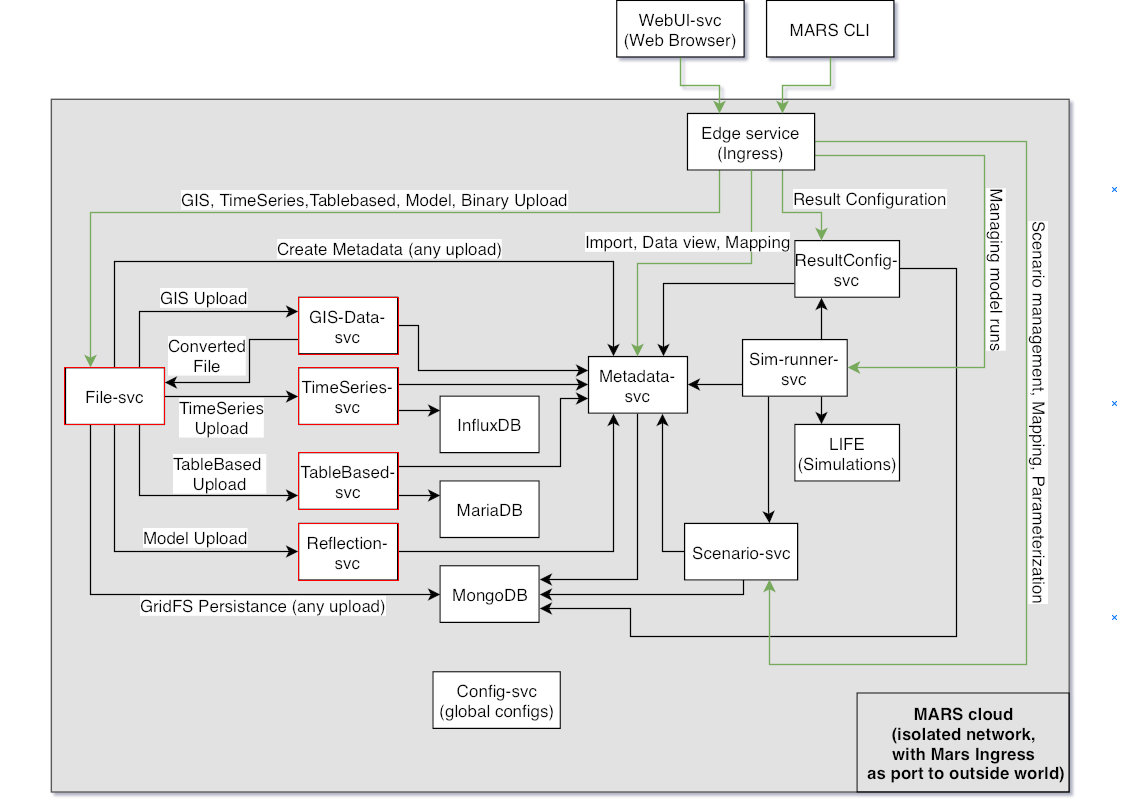
\includegraphics[scale=0.45]{grafiken/mars-cloud.png}
    \caption{MARS Cloud \cite{MARSCLoud}}
    \label{fig:MARSCloud}
\end{figure}

Figure \ref{fig:MARSCloud} illustrates the MARS cloud at the time of writing this thesis. The MARS cloud is a complex Distributed System consisting of many 
Microservices and databases at its disposal. It is a point of interest how the project would be restored back as there are different possibilities for it. 
Although, it is a requirement for the archive service
to call the corresponding service to access add or modify the resources (Chapter \ref{chap:ReqAnalysis}). As mentioned earlier chapters the MARS system
has different types of files (e.g. models, timeseries, GIS) which are managed by their own service. The files can be uploaded in two different methods.
\begin{enumerate}
 \item \textbf{Upload files via File-svc} The File-svc is a service which takes in all kind of inputs GIS, models, timeseries and figures out what type of
    file it is and communicates with respective service for the successful file service. 
 \item \textbf{Upload the respective file via its service} This method requires the Archive service to communicate with each service of the file type. If a file type
 model is to be uploaded a API call to the reflection service has to made and to GIS-Data-svc if a GIS file is to be uploaded.
\end{enumerate} 

The File-svc can be seen as an abstraction layer for uploading different types of files. This layer reduces the number of direct dependencies to the Archive
service because it does not call the other services directly. Choosing the File-svc also provides an additional advantage if a new file type is added in the future.
In this case the archive service does not need to modify any code to upload the new file type. Given the reasons for cohesion and easy maintenance file uploads
via File-svc deemed to be a better choice. 

\subsection{Retrieve as a atomic action}
\begin{figure}[H]
    \centering 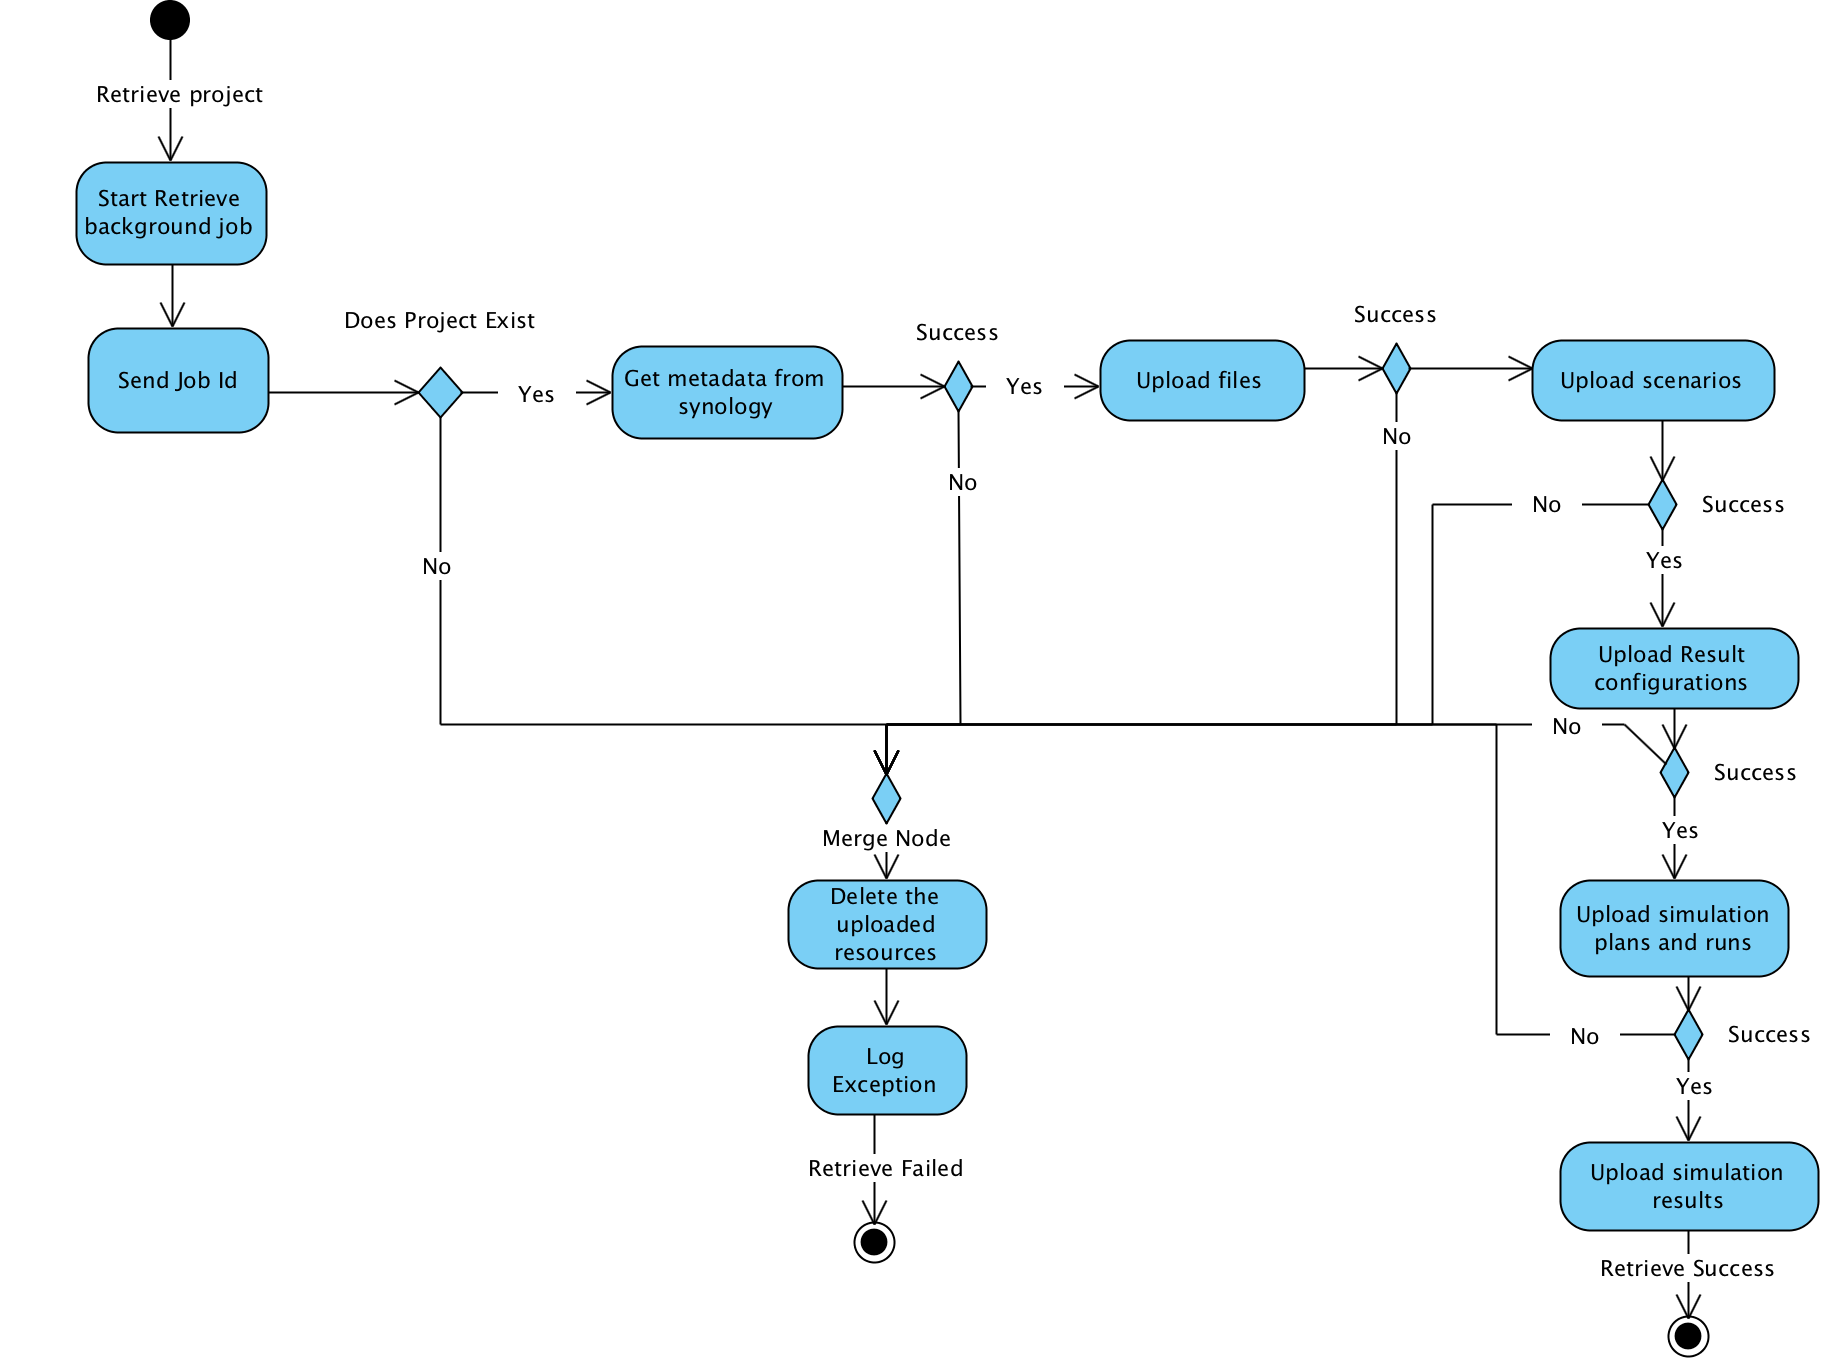
\includegraphics[scale=0.45]{grafiken/restoreActivity.png}
    \caption{Activity Diagram for retrieving a project}
    \label{fig:activityRestore}
\end{figure}

Figure \ref{fig:activityRestore} depicts the activity diagram of restoring an project. The retrieving process is also an background job due to the same reason
as for the archive i.e. long running times. The first step after creating the retrieve job is to get the metadata from the Synology and then upload all the files.
All the files have to be finished uploading and being processed, otherwise the sequential steps would not have the files to use. After all the uploads are complete
the scenarios are compared with the file id for being uploaded. Following the scenarios, the result configurations are also uploaded for the corresponding models.
As the simulation plans is dependent upn the scenarios and the result configurations this is the next resource which will be uploaded. Lastly, the simulation runs
and the simulation results would be uploaded respectively. 

In case an error occurs a Two phase commit protocol strategy is adopted. This strategy is taken into consideration to bring atomicity on decentralized data.
It is always not possible for all the transactions to occur and this would lead to incomplete data restore. In the MARS system one cannot work with having
incomplete data since the resources are dependent upon each other. Having an atomic transaction for the retrieve process would be a simple mechanism to overcome
this issue. In case of any failure during retrieval the successfully restored resources would be deleted to make the retrieve process as an atomic action and
provide a roll back function. 
